\documentclass[12pt,letterpaper]{article}
\usepackage[english]{babel}
\usepackage[utf8]{inputenc}
\usepackage{amsmath}
\usepackage{amsfonts}
\usepackage{amssymb}
\usepackage{graphicx}
\usepackage{makeidx}
\usepackage[margin=1in]{geometry}
\usepackage{setspace}
\usepackage{hyperref}
\usepackage[utf8]{inputenc}

\doublespacing
\author{Justin Zhu \\ Advised by Dr. Alexandre Victorovich Gontchar \\ Written for \textit{Conduct of Life}, taught by Professor Unger and Professor Puett}
\title{The Academy and its Aftermath: Internet Meme Culture and the Subsummation of Liberal Arts Education}
\date{}
\newif\ifdraft
\pagestyle{empty}
\begin{document}
\clearpage\maketitle
\thispagestyle{empty}
\pagebreak
\tableofcontents
\pagebreak
\pagestyle{plain}
\setcounter{page}{1}


\section*{Preface}
In Harvard's Langdell North Hall that iconic portrait of Rosa Parks hangs.  That prophetic gaze is surrounded by that of other notable Harvard alumnus, their portraits impressible, stimulating the better natures of ourselves.  

This is the type of place where great thinkers are created, it seems.

Every Wednesday from one to three, undergraduates, law students, and Harvard affiliates file in for \textit{Ethical Reasoning 20: Conduct of Life in Western and Eastern Philosophy}.  The main attraction is Professor Unger and Professor Puett, two giants in their fields -- their work and discourse complement so well together, I can think of few partnerships that proved so edifying and apolitical.  I was in luck this particular semester because I was taking classes taught by dynamic duos -- there was operating systems by Professor Kohler and Professor Mickens, and inference by Professor Blitzstein and Professor Murphy.  Two professors are indeed better than one, just as two parents to one.  Three would be even more ideal, as Confucius would say.

Unger's fiery bravado and Puett's nuanced polysyndetons bring out the full contrast of human eloquence, played out in philosophical layers.  Considering the class is titled ``Conduct of Life According to Eastern and Western Philosophy," it's tempting to characterize Unger as the ``West" and Puett as the ``East."  Instead, as the conversations unravel onto themselves, one begins to see that the two thinkers share congruent notes on many of the most pressing problems of the human condition, vis-a-vis the ``Western" and the ``Eastern" approach.  

Certain examined truths are timeless, it seems.

As I made my way towards the very front of the room, I walk past the Facebooks, the Gmails, and the Twitters that occupy the screens of those who come in this warm Wednesday afternoon.  As class begins, no context switch occurs -- the cold screens continue to flash the Facebooks, the Gmails, and the Twitters, and Unger's earnest assertions (``Courage is enabling virtue without which all virtues are left sterile!") seems to lose its effect -- the student to my right furtively tags her friend under a meme.   As the professors open up the room to questions, a deadly silence penetrates the musty air.  A few actively answer, but those in the back stare intently on those screens.  Why exactly should we care about great thinkers and timeless truths?  The crickety clicks of fingers to keyboard is enough to keep us all occupied, it seems.

\ifdraft
And I too was one of them, and there I looked, just couldn't help but noticing a certain look in Puett's face that can best be described as pity.
\fi

``God is dead," proclaimed the great Nietzsche.  Is so too the liberal arts education?

\section{The Liberal Arts Tradition}
The liberal arts tradition is perceived to be the gold standard of Western higher education, for plenty of good reason.  A bulwark of advancing human thought since classical antiquity, the liberal arts tradition has served to educate and enlighten individuals in discovering certain fundamental truths.

During the time of the Greeks, a liberal arts \index{liberal arts} education would consist of the core three fields of grammar, logic, and rhetoric, known as the trivium.  Meanwhile, arithmetic, geometry, theory of music, and astronomy form the quadrivium, the secondary fields that comprise a well-rounded liberal arts education \cite{tubbs_philosophy_2015}.  The Latin translation, \textit{liberalis}, translates approximately to ``worthy of a free person," and speaks to the idea of individuals taking part in civic life, becoming good citizens, and living a virtuous life.  

In the United States, the liberal arts education has taken on more nuanced meaning through the years.  A school that practices the liberal arts curriculum in the United States is often perceived as a hallmark of an ``elite education."  Colleges such as Harvard and the rest of the Ivy Leagues have cultivated a reputation that extend beyond just the content and form of education they present to students.  Rather, the sustained liberal arts tradition within these universities have reflected class overtones -- the liberal arts education through much of the history of the United States have often served as a proxy for an expensive and sophisticated upbringing, a symbol exchanged between members of the upper-class to prove that one indeed is part of the upper-class \cite{}.  

This oft-perceived equivalence between liberal arts and upper-class have characterized the university culture much in the United States, as opposed to the European counterpart \cite{}.  The liberal arts culture in the United States has thus served as a bedrock of social customs and tradition, both of which comprise sustained longevity.  The theme of longevity is also a theme consistent with that of a liberal arts education, because the liberal arts seeks to study timeless truths isolated from the rapid changes in the modern world and to use these timeless truths to guide the progression of events in the modern world.

Being said, the rather isolated nature of the liberal arts education from immediate societal repercussions does not merit liberal art's caricature as ``tone-deaf" in popular culture, but rather deserves a distinction of the liberal arts acting as a great stabilizer and social fabric that governs much of the United States.  This stabilizing force is most apparent in the Academy,  the universities and institutions of higher learning that have been around prior to the conception of the United States itself.

\section{The Academy}
If the liberal arts can be described as the verb for advancing knowledge and ideas, then the Academy can best be described as the noun that houses this advancement of knowledge and ideas.

The role of the liberal arts and the Academy is two-fold -- together, they stand at the vanguard of all intellectual and cultural developments, and together, they formalize these developments, thereby becoming the ultimate arbiter over the legitimacy of certain ideas and movements in human history.

Such a great responsibility characterizing the liberal arts culture is appropriate for the Academy, since the Academy often attracts and selects the most gifted and intelligent thinkers of each generation \cite{}.  The culture of the Academy is also one that is isolated from that of pure capitalism governing much of society.  This separation of wealth and knowledge in the Academy has ultimately preserved the inherent integrity and reputation of the Academy just as how the separation of powers in the three branches of government preserved the stable structure and integrity of the United States.  

%The Academy, deemed self-sufficient througgh application, is not at the mercy of 

Moreover, the separation between knowledge and money has never been made more clear for the professors and gatekeepers of the Academy.  The long and tedious path to tenure offers few monetary compensation, particularly in traditional humanities and sciences of the liberal arts institution \cite{}.  Current gatekeepers and devotees of the Academy have been tried and tested, as the path to tenure has effectively winnowed out the individuals who have lessened conviction in their research field of interest and the individuals who have a greater desire to make money.

The Academy, through the trials of history, has ultimately accomplished its goal of promoting the liberal arts tradition, especially in context of capitalism, defined most appropriately as an economic system based on the private ownership of the means of production and their operation for profit.  While members of the Academy often complain of capitalism and financial pressures that affect these institutions of higher learning, history has demonstrated that capitalism is fundamentally compatible with the liberal arts tradition.  In particular, capitalism has complemented efforts in scientific discoveries in the 20th century, as consumer and military interest in mechanized production and innovative chemical and physical resources funneled into more research funding and grants for the theoretical sciences of biology, chemistry, physics, and mathematics \cite{}.  

In contrast to the European model of the liberal arts curriculum, the Academy of the United States have also emphasized engineering sciences to be a major focus of the liberal arts curriculum, as developments in the post-World-War eras sparked much interest in a generation of students who studied mathematics and physics \cite{}.  These developments would later lead the explosion of computer science, applied mathematics, statistics, and engineering sciences in the 21st century, as the world becomes increasingly connected and the era of big data and information overflow alters the dynamics of the individual lifestyle and social landscape to foster more human-computer interaction \cite{}.  

However, while the Academy has historically succeeded in championing original ideas and has led major intellectual and cultural developments, the same could not be said of the Academy today, where the liberal arts culture is no longer occupying a dominant sphere in society.  Moreover, since the introduction of engineering sciences, students have generally transitioned from the traditional liberal arts (humanities, social sciences, and sciences) into the engineering sciences with a particular expanded interest in computer science \cite{}.  Important to note is that the engineering sciences are not to explain for the decline of the liberal arts and the Academy, but rather present themselves as an alternative to the decline of  the liberal arts in the changing social and cultural landscapes of the 21st century.  If the current liberal arts curriculum in the Academy can still accomplish the goals of educating visionaries and independent thinkers as effectively as it did in the past, then there wouldn't be a need for students to switch to the engineering sciences.

Ultimately, the dynamics between the Academy and the rest of society can be attributed to a complex web of factors, but in this paper I will define the Internet Meme Culture that has popularized among the current generation of university students.  Ultimately, the Meme Culture and its predecessors have led to the deterioration of certain liberal arts values in the Academy.

\section{The Birth of Meme Culture}

In 1976, Richard Dawkins published ``The Selfish Gene," explaining how cultural information spreads.  In ``The Selfish Gene," Dawkins coined the word meme as we know it today, which is a unit of cultural idea propagated online.

According to Dawkins, a meme acts as a unit for carrying cultural ideas, symbols, or practices, that can be transmitted from one mind to another through writing, speech, gestures, rituals, or other imitable phenomena with a mimicked theme\cite{}.  As noted by many evolutionary biologists and psychologists, memes have become the cultural analogues to genes, because both self-replicate, mutate, and respond to selective pressures \cite{}.

\subsection{Social Media and Meme Replication}
The advent of social media on the Intenet has contributed much to the rise of the meme culture, enabling mass self-replication, mutation, and response of these ``units of cultural ideas" on a large scale.  As of Alexa's rankings on January 2019, Facebook is ranked the third most popular site, Twitter ranked 11th, and Reddit ranked 18th, \cite{}.  It's also worth noting that YouTube, a video-sharing platform, is ranked 2nd \cite{}.  The way these social media outlets are formatted for short and immediate sensory spread of ideas has become a great incubator for memes.  Twitter limits its users to write up to 280 characters in a single post, while Facebook's Newsfeed contains baked-in stock images and GIFs ready to be deployed at moment's whim.

These social media platforms, having been designed for short messages, images, and clips, ultimately exist as breeding grounds for memes because both social media and memes optimize for simplicity in order reach a broad audience consisting of widespread communication and information exchange.  Just as how viruses contain genes hosted inside hosts, so too do memes contain ideas hosted on social media platforms.  Their gravitation towards simplicity has ultimately enabled memes to gain the widespread recognition it has today.

Simplicity has always been a corollary of evolutionary biology.  The shorter the gene, the quicker the transmission.  Likewise, the simpler the meme, the quicker it's seen.

\subsection{When Meme Becomes Culture}
Dawkins wrote that evolution depended not on the particular chemical basis of genetics, but only on the existence of a self-replicating unit of transmission.  This self-replicating unit of transmission is typified in a particular image and phrase that ultimately becomes planted in the minds of all human beings.  When enough human beings are exposed to this idea to assume an air of familiarity,  the idea then becomes culture.

Dawkins hypothesized that one could view many cultural entities as replicators, and he has listed fashion and learned skills as such examples.  Wigs in the 17th century, for example, were fashionable because people wearing wigs replicated other people wearing wigs.  Meanwhile, learned skills like knitting were popular during that era as well because everybody had to replicate the well-dressed nature of everybody around them.  Today, such learned skills like software engineering are popular because everybody needs to replicate the ability to interact with computers, because almost everybody spends a plurality of their waking hours on a phone, tablet, or laptop \cite{}.

%ecame popular over these last few decades because everybody interacts with a computer.  The amount of screen time on phones and computers have increased dramatically, which is quite remarkable \cite{}.   

Like so, memes replicate through humans, who have, by nature of biological evolution, have evolved as efficient replicators of information and behavior. While humans do not always remember and copy the memes they see perfectly, they exert a considerable aggregate amount of time and energy thinking about memes, engaging in a process of commenting, tagging, modifying, and creating new memes.  Such a process diminishes the individual's ability to formulate original and individual ideas because they are left thinking about framing a particular event with the usual ironic overtones characterizing that particular meme.  By continually spreading memes, the human being becomes nothing more than a host whose mind has become a replication of a meme.  In biological analogues, the mind's cognitive has become infected by a virus, that virus being the meme.

Under this influence of the meme culture, the individual cannot attempt to engage in non-conformity and self-invention, which has always existed as the ultimate question in this project of how to best conduct life according to Western and Eastern philosophy



%Dawkin's formalization of memes and culturesmake 
%
%Dawkins used the term to refer to any cultural entity that an observer might consider a replicator.

%In the 1990s,  a field of study called memetics arose to explore the concepts and transmission of memes in an evolutionary model. Criticism from a variety of fronts has challenged the notion that academic study can examine memes empirically. However, developments in neuroimaging may make empirical study possible.

%they are quite prolific and abundant, reflecting how postmodernism has most notably been prolific with Internet meme culture, a defining movement characterizing the current generation.  Screen time of young people have shared idea,  allart and communication has befound the meme to be the simplest way of conveying information.  A picture and a short caption has proved to be the most efficient way to convey information, and it is this popular meme culture that has seeded itself in the minds of all college students of this generation.  While the colege students themselves havve

\section{On the Nature of Meme Culture}
\label{meme}
The meme culture has been propagated by social media platforms and the inherent evolutionary social tendencies of human beings to replicate the ideas of others.  Just as how evolutionary biology converges on certain optimized, stable states, so too has meme culture converged on certain cultural topics and content types.

To give an idea of the convergent Meme Culture, I have curated a list of the top five most popular memes of all time, according to \textit{The Most Popular Memes of All Time} \cite{}.  The actual memes are listed once more at the end of this paper in order of most popular to least popular.  The themes covered by these memes all contribute to a larger development of Postmodernism, discussed in the next section.

\subsection{Irrational Rage}
\begin{figure}[!h]
	\centering
	
\includegraphics[width=0.3\textwidth]{graphics/2}
	\caption{Y U Know Meme}
	\label{1}
\end{figure}
According to the internet sources, the Y U No meme began as Y U No Guy, eventually evolving into simply Y U No, the phrase being generally followed by some often ridiculous suggestion. The face was taken from a Japanese cartoon and placed on a pink wallpaper, with the initial captions reading “I TXT U … Y U NO TXTBAK?!”  This meme has been ranked as the most popular meme of all time according to Meme Generator, morphing into hundreds of different forms with a similar theme of irrational rage.
 
With arms held out and fingers spread in a plaintive, almost begging gesture,  The Y U No figure stands with looks pained beyond normalcy.  This is a common trope in memes, in that people use memes to express rage over the lack of communication or the little problems that arise in life.   Such memes have resulted in great difficulties for human beings to try to reason calmly and thoughtfully with each other on the Internet.

\subsection{Self-Debasement and Self-Deprecation}
\begin{figure}[!h]
	\centering
	
\includegraphics[width=0.3\textwidth]{graphics/11}
	\caption{Bad Luck Brian Meme}
	\label{2}
\end{figure}

Many memes on the Internet focus on the theme of self-deprecation and the inadequacy of the human condition, and this meme is one of the most popular in conveying this theme.

The Bad Luck Brian meme is used to picture an awkward situation, in which bad luck strikes, represented by this boy who has acne, an awkward jaw posture, and a outdated sweater.  He looks like a very earnest and well-intentioned boy, which makes the meme popular in conveying the inevitable ill-fated nature of our own lives.  Such memes have resulted in a general cynical attitude towards life and the events that unfold in our  everyday lives.

\subsection{Sarcasm}

\begin{figure}[!h]
	\centering
	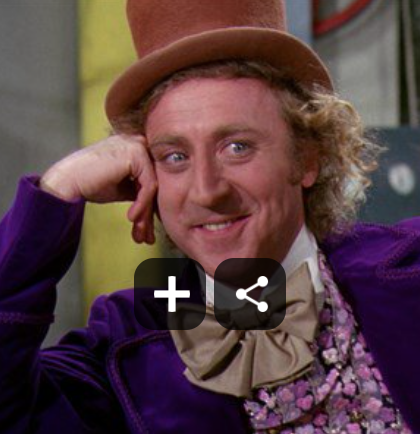
\includegraphics[width=0.3\textwidth]{graphics/10}
	\caption{Willy Wonka Meme}
	\label{3}
\end{figure}

The Willy Wonka Meme represents the entrenched sarcasm that memes express.  This is meme is taken from \textit{Willy Wonka and the Chocolate Factory}, produced in 1971. In it, the subtle sarcasm, most notably seen in Willy Wonka's eyes and Cheshire-Cat-like grin is intended to rebuke earnest statements made by others.  Such memes like these have made it almost impossible for people to express their honest opinions online and live lives genuinely without sarcastic judgment from others.

\subsection{Irony and Boredom}

\begin{figure}[!h]
	\centering
	
\includegraphics[width=0.3\textwidth]{graphics/9}
	\caption{The Most Interesting Man in the World Meme}
	\label{4}
\end{figure}

This meme is taken from the Dos Equis Beer commercials, featuring a live actor playing the role of The Most Interesting Man in the World. The man represented here toughts his extreme levels of interestingness. 

The meme has since taken on ironic meaning, where the interesting is really meant to mask the obvious boredom characterizing one's life.  For example, the parodies that spring up as a result of this ad include the Least Interesting Man in the World, and the Most Interesting Warcraft Player in the World.  This meme has made it common for people to accept boredom as a norm and to use memes ironically.

\subsection{Confusion and Apathy}

\begin{figure}[!h]
	\centering
	
\includegraphics[width=0.3\textwidth]{graphics/8}
	\caption{Futurama Fry Meme}
	\label{5}
\end{figure}

This meme is taken from Futurama, where Fry, the character displayed here, looks confused.  This phrase generally accompanying this image goes as follows: “Not sure if (insert thing)”, with the bottom line then reading “or just (other thing)”. 

The main form of the meme seems to be with the text “Not sure if trolling or just stupid.”  A general sense of apathy surrounds this meme in that people who use this meme generally don't care about which of the options is really the truthful option.  This meme has therefore made it easier for people to perceive the inherent absurdities of the world, while simultaneously encouraging apathetic behavior, where people lose a sense of agency to resolve certain absurdities of the world. 

\section{Postmodernism}

\subsection{Thriving Cynicism}

To understand contemporary meme culture, one must understand the postmodernist culture that has developed prior to the influx of memes and meme culture.  Postmodernism is generally defined by an attitude of skepticism, irony, or rejection toward the meta-narratives and ideologies of modernism, often calling into question various assumptions of Enlightenment rationality \cite{}.  

Postmodernism is not to be confused with modernism in that while both modernism and Postmodernism reject traditional forms of art and culture, modernism at least still retains basic assumptions such as the idea that society is progressing towards a better future and that human beings are powerful individuals with great creativity and ability, capable of changing their environment through the tools of experimentation, science, and technology.  Postmodernism does not assume any of these qualities of society and the human condition -- it looks at the world for all its flaws and accepts these flaws without offering any solution or progression.

\subsection{Relationships to Meme Culture}

The meme culture operates out of these Postmodernist beliefs.  By reading the use-cases of each of the memes under \autoref{meme}, one can gain an understanding of the entrenched skepticism, irony, and rejection rooted in the messages of these memes.  None of these memes offers a solution or a better vision for the future, a characteristic that is distinctively Postmodern.

Postmodernism has thrived as a cultural development in the current 21st century because the 21st century is a time of great propagation of information, the cultural equivalent of the Carboniferous explosion.  The carboniferous explosion is an age marked by an explosion of terrestrial  plant life, and likewise the 21st century is an age marked by an explosion of access to knowledge.  In the age of computers,  globalization, and digitalism, people are disseminating ideas faster than ever through the Internet.  Naturally,  with such an influx of information and ideas, people must exhaust through the baggage of bad ideas that have occurred throughout human history stemming from the Christian-Romantic tradition before coming across some jewels of information that are truly transformative and inspiring.

Looking through so much information and bad ideas leaves people more and more jaded.  Postmodernism channels people's collective general jaded state with more cynicism.  Every idea will have something wrong with it, even if such badness is trivial, as the general cynical sentiment goes in Postmodernism.  

Moreover, the philosophy of Postmodernism is self-sustaining -- one will never run out of ideas to lambast. We can lambast opinions of opinions of opinions of opinions of opinions, and so this meta of lambastment can perpetuate until the last syllable of recorded time.  Postmodernism in this day and age has endless ammunition, ample topics to criticize, and thus, the liberal arts tradition cannot hold out on its own, subsuming and incorporating the forces of Postmodernism.

% more options, more memes, and decide which ideas are worth sharing and which ideas are not worth sharing.    
%
%The 21st century and the world we live 
%A major standard of human vision and of human fallibility.  

\section{Postmodernism Subsumes the Liberal Arts}

Postmodernism's entrenched cynicism towards all ideas naturally translates to cynicism towards all academic disciplines, and so it is this cynicism deeply cutting the very mission and ideal of the liberal arts education.  As stated before, the goal of the liberal arts education is to free the individual by encouraging the individual to explore the very best of what humanity has created so that the individual can pursue larger, nobler goals that will live on past the individual's own lifespan.  Postmodernism has nothing else to say but to point out the futility, impossibility, and faults with such an education.

%A major issue of the liberal arts tradition is that postmodernist culture that stemmed.  
\subsection{The ``Isms" of Postmodernism}
The very nature of cynicism is dangerous because it sparks a defeatist attitude among students, wearing away the intellectual curiosity that is necessary for great discoveries in the Academy and in society.  Such a cynical attitude has coincided with the rise of many ``isms" within academic disciplines, such as Marxism, feminism, and fascism. The branching of many ``isms" in Postmodernism have one general consensus  -- disparage the current system from a particular perspective and interpretation.  Moreover, each of these ``isms" offer no particular solution but an extreme solution that fits the perspectives and definitions of one school of thought.

 These isms are rather dangerous and limited because they only emphasize one particular perspective of the human condition. If one were to declare oneself a Marxist, one can only view the world for all its capitalistic flaws, criticizing the very ``excesses of society" as Marx himself would see fit, harping on ``commodity fetishism" brought about by the bourgeois.  For all the harping, nothing is achieved.  We look to Stalin and Mao and realize the limitations of adhering to strict dogmas and ideologies.  Any ideological movement when pursued with narrow-minded intentions is dangerous.

The very nature of the liberal arts education is one that is entrenched in eclecticism, a certain openness in accommodating the viewpoints, perspectives, and solutions from all parts of life, and it is this interdisciplinary approach that merits much of the great discoveries that have been a byproduct of the liberal arts tradition.  Compared to the ``isms," the liberal arts tradition is more desirable for its emphasis on the universal and the timeless -- what is the human resolve, after all, other than overcoming limitations by supporting each other by doing good work? However, by virtue of it being the historical ``gold standard," the liberal arts stands as the target of all new postmodernist ``isms," and it fights a difficult war along all fronts.  The danger lies in that if the liberal arts tradition becomes completely subsumed, there will be no good alternative tradition that can take on the deep responsibilities effectively that the liberal arts and the Academy have taken on in the history of human civilization.

%Certain truths so characteristic and endowed in our own minds have resulted in these prooat hand where studying the great thinkers of our generation, we come at a loss over hat to bond over, what shared connection that really unites all ofus at the endd of the day.  The great tragedy of the meme culture and postmodernism connects us through the un-satisfaction and imperfections of everyday life.  

% rather than  the heer remarkability  of the life and cultra experiences we have witnesssed within  this generation.

\subsection{Truth}
Postmodernism's inability to accommodate objective truth and its fixation on the lack of objective truth is an inherently defeatist, anti-intellectual attitude, because the truth is really the only thing worth studying at the end.  Postmodernism is an affront to the very liberal arts beliefs of objective truth, timeless truth, as espoused by the Greeks. 

Without a conviction in the truth, we cannot attempt to engage in any deep and serious study that ultimately advances human knowledge.  Nobody can afford to go to University to study the humanities seriously because nobody can truly understand the world for all its faults and beauty by only siphoning themselves with the vocabulary of Marxism, fascism, sexism, racism, and a particular ``ism" stemming from Postmodernism.

Postmodernism as we know it today is an affirmation of our inability to know total truth, dangerous in that it subdues our desire to seek and know the total truth.  

%rather a contradiction against the prevailing ideas of modern society.   Only few individuals have been able to formulate such subjective and objective notions of truth.  We can really see Postmodernism as an active attempt to disengage the mind from the pondering of modern day society.  That to write ,.  There exists a high degree of cynicism within postmodernism that eaves much room to be desired, but I think for the most part our own livves are truly ingrained and intertwined with 

The Academy, having the obligation and responsibility to document discoveries and further the possibilities of the human experience, should not concern itself with the trivialities of the superficial, which is anything that distracts from the search for truth.  However, in the current landscape, the Academy has caved into the demands of a Postmodern world, and the students that frequent the grounds of the liberal arts Academy have only affirmed the deep presence of Postmodernism by actively participating in meme culture.  The ambivalence to truth is perhaps the greatest damage Postmodernism has afflicted on the liberal arts tradition.

%
%For generations, academics devote themselves to a truth, maintaining a conviction in the truth, for this truth is the analogue of divinity in the holy realms of the Academy.  The lack of truth and conviction in truth diminishes the need to study the subject.
%
%.  These pose another problematic issue put forth in university culture.
%
%The liberal arts education has faced intense scrutiny from society mostly due to the



\section{The Decline and Fall of the Liberal Arts Education} 

In the aftermath of Postmodernism and Meme Culture, the Academy has evolved to become a big social club such that the goals of the Academy are not about examining timeless truths but rather about building skill-sets for the workforce.  Due to the lacking of a liberal arts standard to uphold in the humanities and social sciences, students have been turning to the engineering sciences where a standard of truth can be better defined and pursued.  

For those who do not turn to the engineering sciences, they are left to deal with the aftermath of the Academy, this decline and fall of the liberal arts education.   

\subsection{The Arbiters of Excellence}
The Academy's position in society has always been its ability to define the standards of excellence that govern its students, who then go on and impress these standards of excellence within society.  Under this model, the university retains its power on society by the standard of excellence instilled on its students. 

At the very least, this ability to define standards of excellence uniquely positions the University as an institution that is independent and free, one of the very few institutions that do not acquiesce to the capitalism framework impressed on by society.  Losing a standard of excellence in the age of Postmodernism and Meme Culture compromises the very integrity and leverage of the Academy.

In the wake of the decline of the liberal arts tradition in the Academy, two institutions have risen to take on the mantel of power that defines excellence -- the graduate schools of engineering and the corporations.

Today, Harvard's campus rings of recruiters.  If there's any indication of the discrepancy between the power of the liberal arts and the power of the corporations, one can look no further at the students flocking to networking events and socials, leaving the classroom barren.  Only a select few still come to these halls to learn, typing away at their computers,  contracting an attention span that can best be described as distracted.  The goals of the students have been displaced -- academic excellence in the liberal arts tradition has run hollow.

In turn, the graduate schools of engineering have taken on the responsibility to rekindle a safe haven for higher learning, providing a standard of excellence that partially fills the void of a declining liberal arts tradition.  It is a partial void, because while it moves society forward technologically, it can never quite move society culturally.  Postmodernism will still be Postmodernism  with or without the Internet.  Even if better technology was created, people will still continue to converge culturally in the current landscape we see, one of sharing memes with the same Postmodernist themes.  Technology on its own cannot change human tastes and human values.


%To go into research in the humanities is no longer as noble and serious of a task.  Gone are the days of W.H. Auden, who said, ``No, you don't understand.  I'm going to be a \textit{great} poet," when his father asked him how he planned to make a career out of academia.
%
%  As I remember speaking to a Harvard alumnus (who is a neurosurgeon now), he recalled not having any, evoking summers of uninterrupted reading of Milton and Shakespeare rather than an internship at Google and Goldman.  

%Look at any one of the Harvard student's screen during a class and you will notice they are writing emails, texting friends and recruiters, disengaging themselves from the conversation of the classroom in order to find something they don't yet have.  Insatiability, groundlessness, and mortality have long plagued the human condition, and these students, by their own volition and desire to 
%
%Ambitious students who enter Harvard's gates appear to dedicate more time to recruiting for a job than to studying and growing that prescribed wisdom etched on Harvard's Johnston Gate.   
%
%Harvard can also no longer compete with the engineering schools who have made great headway into research
%
%I reembber going intolecture and  facing Unger's most serious face.  The humanities for all its sriving seemstto have made us less sure  of ourselves, where weare in the world.  Itt has certainly made us feel inferior to our senses, to say the very least.  Moreovver, it has also created a  sense of tension, where our inability to come to terms with the rapid change of technology has made  us apathetic and less caring about our own aspirations as indivviduals and peoples of the world.

The state of the current academy is but a dampened representation of the current state of human affairs.  If the students of the Academy have already started to abandon liberal arts in order to scramble for a job, what's not to say that the status quo, deprived of the luxuries of the Academy, are experiencing a even more desperate attempt to conduct lives of purpose in this Postmodern world?

%The ccurriculum in most universities nowadays  cater to the individual who is attempting to thifind some job that can pa off the costts  beared uupon in college.


\subsection{Disconnect with Humanity}
The decline of the liberal arts tradition is ultimately the failure to connect with humanity.  The Academy's disconnect with the working population and the Academy's inability to understand the plight of the American working class is a corollary to the weakening commitment to civic life established in the liberal arts tradition.  

%The Academy has always been a champion of the working individual 
%
%The greatest failure of this state of aftermath characterizing the decline of the liberal arts tradition is the Academy's disconnect with the working population and the Academy's inability to understand the plight of the American working class.  The Academy has always been a champion of the working individual.
%
%This disconnect is due to the changing

The very definition of the Academy has changed.  Rather than serving as bastion of liberal arts education, the Academy now acts as resume rubber-stamps, a place where prestige floods the area but emptiness walls the innards.  People tout their status of being a college graduate, but few truly have something to show for it.

This realization is frightening for many people, who took out loans and the best years of their lives to pay for this certain emptiness.  They adopt some variant of Stockholm syndrome and glorify their college years, and then look down on those who did not go to college as an inferior breed.


%While those who remain in college and do not pursue the engineering sciences in learning a trade, look down upon the working-class who did not go to college.


%Such a frightening prospect for human condition takes a toll on individuals.  This is where individuals truly begin to fail to see he distinctions that characterize what many know to be the end of the liberal arts tradition.

%The key aspect of  liberal arts education has really been to produce individuals with great  civic virtue
%
%There is a vast impact on American society and the intelligentsia, the foolish attitude of the white, working-class who did not go to college.  
%
%People don't take out their IQ scores.
%
%The way people think about college is "He want to Harvard.  He must have been very smart."  This right-wing figure were over a conflict over a film.  This person said to Jeremy, you didn't even go to college.  People who go to college feel like they are more privileged.  The person who went to Yale is smarter than Junior college.  It is not universally true, it does not translate over to a level of success.  Innate ability does not translate to ability.

%People can brag about where they went to school.  Most of us have institutions.  Church and work.  Their social fabric is created by them working with others.  School or church.  As churches declined and as schools become less of a binding commitment, the social fabrics disappear.  Colleges have become a new social fabric.  

There has been a rising sentiment among college students after having attended liberal arts institutions to look down on those who are working hard to pay the bills, the people who have deferred the opportunity to attend college during this juncture of their life.  Not having gone to college is frowned upon, but what really is so special about this degree that individuals emblazon on their screens?

Connections, one might say.  But what connection is there other than the \textit{human connection}, the overarching connection that unifies all of us rather than an exclusive few?

The connections that the Academy claims to bestow upon its students (a rather cheap substitute for the liberal arts tradition) is not a connection at all but a division between those who have gone to college and those who have not gone to college.  This type of division is the type that has translated directly into the problems we see today.

Those graduated with a college degree dictate the division between college and non-college.  Those graduated with a college degree take arms against working-man, throwing slurs like racism and sexism, casting away the humanity of the working-man in the delusion that they are serving some greater humanity other than the one they've been seeing this entire time.

This alienation between the Academy and the working population has ultimately made the working class grow distrustful of the Academy, for good reason.  Out of spite it seems, the working class has turned to right-wing populism, not because it is the best solution but because the alternative civic life that extends the liberal arts tradition simply is not there.


%There is no better or greater solution for these people.
%
%
%
%in the aftermath of the liberal arts tradition has alienated itself from the many troubles of the working population.  
%
%The visible disconnect between the Academy and the plight of the working man has lead to the rise of right-wing populism.
%
%, turnning away from the plight and suffering of the working man.  Such an attitude is deeply dangerus and contributes t the overarching image of the arrogant and supercilious educated man.  In fact, the very nature of colleges has become some sort of social emblem.  When people say they did not go to ccolege, employers.  
%
%A useless degree has been the resut of this world, and people ride the coattails of the liberal arts education, it name rather than its nature.  And so too has this generation evolved amidst the waves of .

%something that is entrenched in the liberalism of past generations, something that modern individuals cannot fathom or hope to fathom iin this day ad age.

\section*{Tomorrow, Tomorrow, and Tomorrow}
As the last class concludes, Unger remarks humorously to Puett, ``And so here we are, discussing the most pressing problems of our time, in a hall that is somewhat fit for a discussion like ours."  

The irony was not lost on me, but was this really irony, or had I been too disaffected by the Meme Culture to even recognize a display of raw, true human emotion?  To be human is to be vulnerable, and here I was, seeing two Professors laughing together like schoolboys.

Perhaps it is too premature and sensationalist of me to write off the decay of the liberal arts curriculum as if it were an empirical fact, as many of my predecessors have done so in the past.  The statistician in me asks, is this decay measurable?  What is a good confidence interval for the years the liberal arts has left until it dies?

For all the statistics, computational models, and math I've learned, at the end, I admit I do not know other than the fact that I am a Romanticist at heart.  Such a statement would never fly by today in this world of machine learning, big data, and data science, but I look upon these walls with nothing but a feeling, an impression that something magical still lives on in these gates as they did three hundred eighty-three years ago.  

As I write away this essay, a young pre-frosh asks me.  Is it true that Harvard is now known as the Stanford of the East?  We live at a time of great technological change where Harvard is known as the ``Stanford of the East," which is not an affront to Harvard or to Stanford, but to the explicit infallibility of the liberal arts culture and the human tradition giving way to engineered systems and machine learning.  We are not as ``sophisticated" as we make it to seem.  

But I smile.  ``Let me show you something."  


I have looked upon the midway mark of my college years as.  Ceaselessly, I go on, excited to see the newest wave of statistics and computer science meshed with the pure sciences of biology, chemistry, and physics, but I do admit the philosopher, writer, and humanities, as with many others.  

As I type away, 



I think about a certain possibility of humanity, of Shakespeare, and of 

.  But they will teach this class next year, and perhaps the year after that.  What will change?  

As Shakespeare duly noted

Tommorow, tomorrow, and tomorrow,\\
Creeps in this petty pace from day to day

many rows and rows of students whose eyes dart forth on their laptops sprawled with Facebook, Gmail, and Twitter.  This is the world we live in, a time where the distinction between work and play blur, and the precious seconds of our lives are spent.  

Notions of the self are changing, and this is the paradigm that has made us increasingly less hesitant that we know what we are doing than to doubt our inability to do it successfully.

To reclaim the liberal arts tradition at this point may be a futile endeavor,
as the changing nature of the times calls for people to be more oriented around computers and the Internet in proceeding with their lives.  We live at a time of great technological change where Harvard is known as the ``Stanford of the East," which is not an affront to Harvard or to Stanford, but to the explicit infallibility of the liberal arts culture and the human tradition giving way to engineered systems and machine learning.  We are not as ``sophisticated" as we make it us seem.  

What should we do about the Meme Culture?  What should we do against Postmodernism?  These are questions that we will perhaps never find a satisfactory answer to, for good reason, because the answer may just not be there.

To infuse the liberal arts with new meaning, to let it, metaphorically say, take on the wings of a butterfly after shedding its exoskeleton as a caterpillar, that seems to convey the full extent and capabilities of the liberal arts curriculum.

Looking at the current way classes in the Academy are structured, where students have complete access to personal laptops and phones housing the Internet while class is in session and the professor is speaking.  The lectures are recorded, which further disincentives students from coming to class and contributing meaningfully in section.


and many students have found themselves at a loss for deciding

Most students have evolved to the point 

sacknowledge that class participation 

The Academy no longer impose a standard of excellence where the student is 

The Academy has become a busy hubspot for 

It doesn't come as a surprise.  The liberal arts.  Part of the fascination with corporations is that they have logos, those picturesque pieces of, or that certain ``hue of blue" (referring to Goldman Sachs or McKinsey).  With no measure of true excellence endowed in the academic sphere, ambitious students search for excellence in other areas, which certainly falls in the.  

These logos of corporations have themselves been part of the meme culture.  Google's very own ``Google for Doodle."  Forget about surrealism or the arts.


\subsection{Standards of Beauty}




It doesn't come as a surprise.  The liberal arts.  Part of the fascination with corporations is that they have logos, those picturesque pieces of, or that certain ``hue of blue" (referring to Goldman Sachs or McKinsey).  With no measure of true excellence endowed in the academic sphere, ambitious students search for excellence in other areas, which certainly falls in the.  

These logos of corporations have themselves been part of the meme culture.  Google's very own ``Google for Doodle."  Forget about surrealism or the arts.


The Academy has become a start-up incubator and places of networking, losing a certain soul in its mission to uphold the liberal arts tradition.


In turn, society and employers 

Moreover, universities have, alienating themselves from the working class.  This has led to the rise of right-wing groups.
Instead, universities are prioritizing credentials and big social clubs. 




The death of the liberal arts has in many ways been attributed to faults of the society giving way to technocrats.  Human connection is fallible and without the understanding of human connections, as Shakespeare formalized it in the his era, it would be impossible to do without the other things that make the liberal arts so successful.  After all, the liberal arts is so characteristically human, that is it is built on the ideas of human advancement, celebrating individual thinkers the unique human beings that embody the highest forms of ideals we all strive for.  Moreover, it is a testament to the spirit of the human resolve, where taken back by disadvantages, whether these deformities are physical are natural, human beings cantill gain a better idea into wha is at the end of their life, the own recourse by which we are striving to learn and breathe and feel an invincible enseof connection.  these disadvantages have ranged from the physical (Beethoven's deafness and Stephen Hawking's ALS) and also the dsocioeconomial 

The memes culture often employ a wide arsena of tools of iterary tropes.  There exists the ironic trope, there alwso existss onesthat seek to refirm cultural identities, very much ironic because theaffirmmatn of ccultural identities can be interpreted directly to racism if the cultural identity does  not desccribe the individuall.  Certain truths so characteristic and so el-endowed into our own minds have resulted in these prooat hand where studying the great thinkers of our generation, we come at a loss over hat to bond ovver, what shared connectionthat really unites all ofus at the endd of the day.  Such is the tragedy of the meme culture, it builds on this postmodernist angst onnecting each of us through the unsatisfactionand imperfections of eeryday life  rather than  the heer remarkability  of the life and cultra experiences we have witnesssed within  this generation.  

To characterize the liberal arts education as ``dying" is perhaps a bit of an exaggeration.  Throughout much of history, many academics have bemoaned the sorry state of liberal arts as we know it, but statistics have proved otherwise.  In the Ivy League universities, for all their curriculum changes, have maintained a strong and stable humanities student population throughout much of the 20th century.  However, entering the 21st century, a noticeable transition has occurred where students no longer study the humanities and arts that usually indicate a strong liberal arts tradition.  In Harvard, for example, the number of English majors have been a third of what it used to be.   

Finally, with the air of postmoderism, therere is an emphasis of framing the problem rather than alternative solutions.  A major precedence in the university culture has been the rise of right-wing populism that hae stemmed from a certain disonnect between the university ttraditionand that of its c..  The univerity culture as a result of this postmodernism, isolated itself from the many troubles of the working population.  Those who have gone to college have often looked down upon the working-man, throwing phrases like racist and sexist upon lower-class members, turnning away from the plight and suffering of the working man.  Such an attitude is deeply dangerus and contributes t the overarching image of the arrogant and supercilious educated man.  In fact, the very nature of colleges has become some sort of social emblem.  When people say they did not go to ccolege, employers.  A useless degree has been the resut of this world, something that is entrencched in the liberalism of past generations, something that modern individuals cannot fathom or hope to fathom iin this day ad age.

The problem with relaxing standards  and grade inflation is that it boosts the ego of the man


There is no stakes for the individual when he is commenting on the works and endeavors of the other individual, where society immediately shuts down the efforts of the artist, deeming the art offensive, as such an effort has led to the creation of many, multiple 
With such self-censorship in mind, the artistic culturehas developed into a rather.  Not to sound like a snob, but I think there exists a signifiant different between Kany



In order to understand the present-day meme culture, we have to understand postmodernism.


Having spent a good portion of my personal time perusing and analyzing these memes (I made the decision to curb my usage there

The great secularists of our era, the notion is often said that individuals  who are exposed to the corruption of he youth often fare without other intensity,most certainly the way our own ideas are cafted amdist the wonders o the world.  It i ultimatiely a tragedy in the end when things just do not end up the way they should be, and thss isnot the byproduct of Kantian ethics but rather the limitations  of postmodernist worlds.

whereas  the culture of humanity has been loosely interpreted to mean aweak loose  interpretation of the world at large, this is not entirely divorced from what is the true  moralhigh ground, the true high path.  This high path is one where everybody is not entirely sure where to go, wheereto proceed,  and it's something I'vve found distressing over the time atHarvard/  Sometimes it is the eleemeental effects that take hold of our opinions that  prved the most deafening for how we are to perceive  the world for wall it's meaning.

Uagine we have something likea  post

EQUATION

Certainly other setups are valid and almighty, but none  really compare to the one I feel and see, which is the segregational conjuring of human voices, drowning out the noise.

So what to do?  Mems and high intellectual culture will never seem to end, while other aspects like coding will not seem to  exist anytime soon in our cconjuring  of  other  methods of files  and sk systems.  To write good code ultimately requires an understanding of the basics, readinggood code, and not being afraid to write the cde down.  Only then wiill  individuals have a better understanding of productivity in the midst of greater awakenings, for the mind of the coderis then released and bolsteredamidst the onset of newe greater difficulties that stem beyond the originalchallenges at hand

Origins of meme culture...
these  issues are very much ingraned in the culture of human ides, and human suffering.  

The meme culture has subsumed much of the liberal artscultur, because it has largely repplaced much of the nuances and intracies of the human connection.  It is not an uncommon  sight nowadays to look at young people in the world and remark that feel that 

However, To ``obtain a liberal arts education" in American often means establishing elitism.  Proponents of the liberal arts education have endeavored to call out the entrenched elitism.  However, while the liberal arts.  As Nathaniel Hawthorne would say, ``Families are always rising and falling in America."  These sentiments run quite true in today's era of 

The liberal arts curriculum as we know it today is one where we havve not yet formaized orddiscovered the truly productive tools needed to make gacy.  The critics of the Postmodernist age have characteiized it as such.  Our own musings is very much unprecedented, and our thoughts like the bubbles in which we have stopped to think as also highly anticiapted.  It does not even matter how do we conjoint het ways of thought in reclaiming our heartland, as Slaman Rushdie once ssaid, but it's more about reclaiming a certain kind f art, one where we are turly enamoured and conjoinedin seizing our own individual experiences.  This to me formms the bulk of my own existence my own vvision for how the wk in the turbid ebb and fllow of everyday life.  To discover the worl as I see it, and to make use of it for deeer insight.  That thought is so liberal arts.

I think this is a prettycool idea if we want to isolate the signal from the noise  I've always been vvery interested in these type ofhings, realy speak ts to the high quality  of reports being created during this time of period


s
The problem also ariees with theformof the ``met`` culture within  the meme culturewhere individuals contnue to lambdast 

However, in this modern Internet culture, the social significance of the liberal arts becomes much more subdued, which takes away its power and relevance as in society as a vehicle for ideas and social progression.

With its social significance and historical roots established in the context of the United States, the quality of a liberal arts curriculum has had various levels of success, but a general trend from postmodernist culture have largely diminished the reputation of the liberal arts curriculum, to be discussed in later sections.  Being said, the typical model of the liberal arts curriculum still deserves much of its quality from the Greek traditions, living up to a certain ``gold standard" that have stood the test of time.  It's not so much that the liberal arts culture has been endowed with certain qualties that .

, adding to the very definition that life is inherently short-lived and.  Stemming from 

The path to tenure has been increasingly tenuous.  Research funding tin the humanities have decreased In the Baroque era, the church was known to serve as the main patron for the arts, the classical era had more of ciprorations contributing to the world at large and finally, the cassicall era has seen more our own development in context of capitalissm serving as the main patron for theibeeral arts.



There is also an interesting overtone to which the liberal arts education can be perceived as deceiving.  I dor onw have often realized this to be the case, that our thoughts are foten enjoined with the prospect that life, no matter how short and unrefined, still  have other fac

as I defined in my first paper, ``Self-Reliance in the Digital Age."  The class, as with all other classes at Harvard, adopts a very lenient policy

Such a scene expresses the liberal arts culture as I experience it now, as an undergraduate who once had some aspirations to leave my mark to humanity in the humanities.   



They click on thumb icons, heart icons, tagging their friends on Facebook.  A conditioning that is inevitable, but also as a way to express ourselves and assert our existence.  The power of the Internet is its connection, and it's this connection that fills me with great optimism for the world ahead.  The marked departure to the very ideas expressed by all of us.  These are the essays that define our generation.

Looking at the students 

The sight of an entire auditorium nowadays sprawled with new is not an uncommon sight.  The content of these screens is furthermore interesting.  We can examine the psychological narratives of our own world departing from the limits of the human imagination, that is, wes

As class starts, no context switch occurs -- everybody proceeds to refresh their screens, checking the NewsFeed on their Facebook profile.  While they might.  These images are some of the 

the content of Puett and Unger are rapidly profound, the effect is not particularly so.  

Few were taking notes on their MacBook Pros, and there was not a single screen where I did not see Facebook, Gmail, or Twitter occupying a third of the screen.  I defined in my first paper, ``Self-Reliance in the Digital Age," that the underpinnings.


\section{The Academy}
I reembber going intolecture and  facing Unger's most serious face.  The humanities for all its sriving seemstto have made us less sure  of ourselves, where weare in the world.  Itt has certainly made us feel inferior to our senses, to say the very least.  Moreovver, it has also created a  sense of tension, where our inability to come to terms with the rapid change of technology has made  us apathetic and less caring about our own aspirations as indivviduals and peoples of the world.

The state of the current academy is largely reflective  of this current state of human affairs.  The ccurriculum in most universities nowadays  cater to the individual who is attempting to thifind some job that can pa off the costts  beared uupon in college.

The very definition of the academy  has been changed.  Rather than servving as bastinos of liberal arts education, universities now serve as start-up incubators and esume rubber-stamps,   place where prestige lfloods the area but emptinessswals the innerads.  Such a frghtening prospect for human codition takes a toll on individuals.  This is where individuals truly begin to fail to see he ddistictions that characterize what many know to be the end of the liberal arts.

\section{Beauty}
It is interesting to examine popular meme culture and juxtapose the culture of internet memes with the subsummation of the liberal arts culture because both entitiees have some element of beauty entrenched in its very rooots.  Seeing that beeauty itsef is subjctive,we  cannot ayy if mem culture truly is i%nferior towhat has associted tobe standard fare of the liberalarts, which typicallly consists of the canon of Davinci, van gogh and picasso.  

We can look at the culture's realation to beauty to understand more about the state of affairs that occupy the minds and thoughts of the people of its  culture. That's what makes this piece so endearing.  It's the very thought of greater moral striving, the unanticipated good over the face of eveiil that makes  us more inquisitive and curious to see what everythig isabout.  This feelling is one that is fleeing but it makrks a unique insight intothe very nature of cultural differences and unique sufferings.Take a look at the following  meme samples one can get a basic sens of what  ailmets characterize youn gmemers today.I remember distinctively as a, eager to drink deep, lest I taste not that Pierian spring.  I was shocked when Professor Unger in the very first lecture of the class immediately.  If philosophy, the mother of all humanities had descended into death, then how can I truly have witnessed the own subsummation of my own culture and my own anticipation for the way things go?

 What I witness everyday is the Internet Meme Culture, and the subsummation of the liberal arts curriculum.  Just as Modernism defined and, the current post-post-modernist landscape is captured best by machine learning and memes, a cyclic loop of content and optimization, leaving little room in the liberal arts.  A whole generation staring endlessly through 




\ifdraft
My class schedule this entire semester had taken on an interesting flavor -- it was going to be taught.  The benefits of, it's like growing up with two parents who aren't divorced.


I can name of few dynamic duels that I know off -- Joe Blitzstein and Susan Murphy in the Statistics Department, James Mickens and Eddie Kohler in the CS department, whose operating systems class starts at three that very same day.
  \fi


The class is ``Conduct of Eastern Philosophy."  Ooh, I should try it as if it were some type of East Asian delicacy.

This place in the year of 2019 tells of a distant story.  Shelley's Ozymandias poem.  Look upon ye mighty and despair!  And this has been the general sentiment.

Yet, a friend of mine Gabriele.  Want, He's a good friend, and I will certainly chanting Hebrew on Saturday mornings when I think about my time back here at Harvard.

A certain type of gloom hangs in the air.  Philosophy, the mother of all humanities sounds nothing but a sound of platitudes.  

Unger bellows, ``Courage is enabling virtue without which all virtues are left sterile!"  Besides me, a student refreshes Gmail.


 Such a scene would make anybody exclaim, ``Wow,  This truly is Harvard."

For example, a portrait of Rosa Parks hangs in the amphitheater surrounded 

\section{The Liberal Arts Tradition}
To be fair, Harvard was never particularly successful in getting its general education system up and running.  In 1916.

Drew Faust

The uniqueness of Harvard's liberal arts tradition has always been to cultivate ``gentlemen-leader of the world."  In the current post-modernist phase, we would be quick to point out that now know under, a very gendered term and also very colonialist, and colored by capitalism overtones.  But such a critical attitude breeds cynicism.

\section{The Internet Meme Culture}

Faust left for Goldman Sachs.  The irony and literary allusions surely did not leave us.  The meme culture.  A cultural tradition has always been dependent on shared appreciation.

.   It's the six.  Unger bellows into the air.  It's somewhat unsettling that the very auditorium, a certain despondence hangs over the classroom.  This is a class with law students.  I peer over, glancing.  Beyond me, another student copies and pastes his resume onto his LinkedIn profile.  All seem impervious to the lectures of 

It had been a Harvard I had seeking.  Going about.

Harvard, the vestige of high American culture, high world culture seems to run hollow these days.  God is dead, proclaimed Nietzsche, and perhaps too is the liberal arts curriculum.

\section{A Time of Recruiting}
It doesn't come as a surprise.  The liberal arts.  Part of the fascination with corporations is that they have logos, those picturesque pieces of, or that certain ``hue of blue" (referring to Goldman Sachs or McKinsey).  With no measure of true excellence endowed in the academic sphere, ambitious students search for excellence in other areas, which certainly falls in the.  

These logos of corporations have themselves been part of the meme culture.  Google's very own ``Google for Doodle."  Forget about surrealism or the arts.

One is left to wonder what is the state of the liberal arts curriculum in this day and age, whether any of it exists at all.  The influx of computer science [insert citation] moreover, is illustrative of a larger issue that the liberal.

\section{Asian Culture}
Another point I would like to expound on is the Asian culture, which has always been copy what works and then make it more efficient.  This can be seen in the.  Western paradigms of artistry and individual ownership of work are not pervasive themes in Asian culture, which I should discuss mostly as culture in the Chinese, post-Mao tradition.  Mao's influence on China has one that led to a ``survivalist" instinct in the masses.  Those who survived.  My grandparents have been very reticent about this time in their lives, and from what I gathered, it has been no different from Cormac McCarthy's \textit{The Road}.  When I return to China, I have often felt.  My friends often asked what China was like.  

Imagine capitalism without Christianity, I said.

I bring up Asian culture because it largely reflects my own.  I have always identified as Russian, since my mom was raised in the very northern regions of outskirts.  While it is the last names of our fathers that we carry in our names, it is the soul of our mothers that we carry in our lives.


\section{Shakespeare and the Humanities}
Harold Bloom commented on 
I originally planned to concentrate in English because it represented more of my own personal 

We are left to ponder what then consistutes the formation of the self.  Individuals like Hamlet.  The problem with Hamlet is that he doesn't say what he means and doesn't mean what he says.  And I too, like Hamlet, have found myself at odds with myself, purporting that I embody a certain sophisticated individualism, while at the same time recruiting shamelessly for investment banking firms, hedge funds, and big tech companies like many.


\section{The Post-War Asian Culture}
Puett describes.  

But this is no counsel of despair. In 1773, Samuel Johnson visited the University of St. Andrews on his journey to the Western Isles of Scotland. St. Andrews is an ancient institution, one of the 25 or so oldest universities in the world, and yet 350 years in, it had evidently fallen on hard times. Fewer than 100 students remained, and one of its old colleges had been dissolved. "To see it pining in decay and struggling for life," Johnson noted, "fills the mind with mournful images and ineffectual wishes." He was under no illusion as to where the blame lay: "It is surely not without just reproach, that a nation, of which the commerce is hourly extending, and the wealth encreasing ... while its merchants or its nobles are raising palaces, suffers its universities to moulder into dust."

The humanities and the university do need defenders, and the way to defend the humanities is to practice them. Vast expanses of humanistic inquiry are still in need of scholars and scholarship. Whole fields remain untilled. We do not need to spend our time justifying our existence. All we need to do is put our hand to the plow. Scholarship has built institutions before and will do so again. Universities have declined and come to flourish once more. The humanities, which predate the university and may well survive it, will endure — even if there is no case to defend them.




\section{The Academy}

The arguments being made have to do with a particular area of our experience.  As the argument becomes comprehensive rather than provincial, dealing with the hole of our situation, the distinction between the is and the ought breaks down.  Indeed we can apply this to the claims of the philosopher David Hume, who in his treatise on human nature presents a view that is at one descriptive and normative.  A second or third characteristic of these orientations through existence in this space in which religion and philosophy merge is that the argument in favor of taking one or another position always seem to be disproportionate and inadequate to the weight  of the choice.  No other choice is as important with what are we to do with the only life that we have.  Within this contest of visions and orientations, the arguments never seem to be conclusive.  There is a frailty given the faithful weight 


The liberal arts curriculum is one often represented by multiple stages of human underpinnings.  The motivation, life as we know it is propelled into something deeper, more elemental.  Such are the purpose.  This paper is a dedication to a journal, manifesto of personal philosophies compiled and influenced by Nietzsche, Schopenhauer and other notable thinkers.  It is a tribute to the idea of human striving, of the mere ``essentials" of life, of tasting the bare essentials of life.

A major question has always been the purpose of the academy, of higher-education, the very liberal arts curriculum that an individual undertakes during the formidable years of college.  This education is formidable because it marks the supposedly complete maturation of the self, one where the individual will have explored deeper ideas of his own identity and personality.  The thinking goes that once a young individual is able to fully identify his/her own identity and personality, the individual will be able to identify .  The job market comes and goes, with new jobs created and destroyed all the time.

\section{Sun Tzu: The Art of War}
The Art of War is pretty important in that the individual is able to internalize something more 

\section{Youth and Self}

The youth is what is most impressive, characterizing the most important attributes of human surroundings.  Sometimes I woder who I am, the effusive underpinnings, lost in thought.

\section{Relationships}
The Confucius tradition necessitates a certain grounding of truth, where individuals are.  Confucianism is a broader set of ideas where individuals are compelled to look upon

\section{Individualism and Self-Reliance}
This is the individual and self-reliant perspective, where individuals are able to internalize and describe something more fundamental.  Individuals are able to internalize and describe the world, seeing a more versatile literary style.  People are more contrived to explore other pathways to human understanding.  My own personal manifesto.

\section{Work and Family}

\section{Romance}

\section{Relationship between is and ought}

\section{Reclaiming Humanity, the Liberal Arts, and the Conduct of Life}
Arguments have to do with a particular area of our experience.  As the argument becomes ccomprehensivve rather than provinccial, dealing with the hole of our situaation, the distinction between the is and the ought breaks down.  Indeed we can apply this to the claim, with the philosopher David Hume.  He himself in his treatise on human nature presents a vview that is at one descriptive and normativde.  A second or third characteristc fo these orientations through existence in this space in wchihc religiona ad philosophy merge is that the argument in favor of taking one or another position always seem to be disporportionate annd inadeqate to the weight  of the chioce.  No other choice is as important with what are we to do with the only life that we have.  Within this contest of visions and orientations, the arguments never seem to be conclusive.  There is a frailty giiven the faithful weight 

The cognitive gap.

The implication othe cognitive gap is what we make what Pascal has called the wager.  We us take a risk with incomplete insigt about the most important matter.  There is no wayof overcoming that.  This gap exists in Western theology as faith.  Now,

The demand for this wager is another form of faith or trust.  As we act on the basis of thesepositions and ideas, fo which the justification never seems to be suffcient, we become vulnerable or morevulnerable to the others.  This heightened vulnerability is a consequence of the need to risk ourselves.  The sapce i we conduct this inquiry.

Fourth characteristic 

These orientations through existence whether represented through religion, philosophy, or marriage ofthe two, ccannot be cabined in a narrow slice of life.  Each should penetrate the whole of existence.  It's interesting to reflect on this historically because religion is a coinage of the 18th and 19th centuries and associated especially with the middle period of the history of Protestantism.  This was the period in which the dominant ideas in Protestant Christianity as the private conscious of religion.  Not a project that informs the whole of cocllectie life, not  characteristic of Luther and Cavin.  Tis is not a coomponent to modern Protestant theology.

Political thinkers like Maidson repesent a anomaly in the history of theology, but that's where the word religioncomes from.  We are misled by the geneology of the privitzation of religion, sacriligious because it doesn't address the complete socialization of llife.

Now, to  make a seond set of remarks, the shared characteristics of these dominant orientations that move through existence, originatingthrough a series of religious revolutions that mar the human history fro 1st millenia to after the 1st millinia after Christ.  These expansions of religion includde what made from a Western view to something else entirely.  Buddhism and iits pecursors in ancient India and Confuccianism in Chian.  Even after we expand radicaly the concept toaccommodate all of these orientations, what is striking is despite their vvery real differences, there are certain common traits among these orientations originating from these spiritual and religious experiences from the past.

The commont traits are:
1. The decisive repudiation of ccosmothogism, the santity of religion, the natural world is sacred.
Thesacred is defined as being in tension with the workings of nature, something utside, whether something is outside, the intrapersonal or the interactions between the transcendent god and humanity, a dramatic dialetic between transcendence and images, teh devine betwyond nature andd the presence in imminence.  Each of these orientations represent this ddialectic between transcenddence and imminence.

222nd orientation is that th focus ofthei oncern changes.  It ceases to be ur dependence upon the powers of nature and it becomes the basic problems of the human condition.  Our groundlessness and insatiabiity.  The fundamental questionis how we are to respond to the question of nhilism, the fear that the world and our existence  in it may be meaninglessness.  There is no meaning to the terms in how they are trasnlated to us.  Eacch is a response to the fear and danger of nhilism.

A thir ccharacteristics, the dv, the divisons of cass or caste.  These divisions are shallow
Retains it's imprints like Plato.  There are two parallel hierarchies in this world.  

There is a social hierarchy, down below there are the workers, the hierarchy corresponds to the hierarchy in the soul, the sensual appeptites, and the most important row of philosophy is a way of thinking that allows us to recognize the significance of these hierarchies and rject them.  In favor of these views of the unity of mankind by all of these orientations.  Then comes the fourth -shared characteristic is the substiuttion of the ethic of the rulers and of martial valor.  A proud self-assertion and of vengeance.  In facor of fellow feeling or compassion.  The contest of these visions are altruism , standpoint of love.  the etic of self assertioniis immediately plausiblee, an existential bsi, that we can describe it as the ethic of ltitle voice.  This is the ethic in the history of humanity.   It's astonishing that the ideas have penetrated so many civilizations and triumphed in what we regard as ripe or deep.  

The ifth common characteristic is that there exists an ambivaleence with respect to their relation with the woorld as it is, th social world.  Are we to take them as redescrptions of the world or invitations to change the world?  The proposition that the humanity are shllow and don't goo all the way dwn.  The sve and amster are ultimately in the same level.  Are they uultimately in the same levell, or do they apply to the abolition of slavery.  Thereis a licese to escape from the world to anotehr world that wil not exist here or now and we think that history is a nightmare from which we want to awak, that is one interpretation, the other is that it must be now or soon and that there is not a ticket to escape but a command to transform.  Ths is an unresolved ambivalence in all of hese views.  All of them in their historical relaity as they have evolved in the world have enteredd into compromises and transactions with the regimes in the world, copromises that deny the transformations intthem.  The impulse to transformation has been inhibited in two opposiing ways, the religion of the law and the religion of he heat.

Fixed normative orders that serve as a proxy through the transcendent, as a kind of freezing of the dialectic between the trannscendent and the imiminent.  The religion of the heart is the internal experience iin the priate conscious directly related to the divine.  This is possible with whatever happens in the world.  This is another way of disposing of the problem of this two-way ticket to escape and transformation.  Examples can be found in the religion of the law and the religion of the heart tot he conduct of the life. 

A question raised is what about us in relations to these historical developments?  Do we have to combine them in some way to to establish some sort of synthesis or canwe take them in points of departure for another spiritual revolution?  Are the gates of prophecy closed or are they open foreve.  It's a question of vast significance.  The gates o fprophecy are open and religious revolution are something for now and not in the past.  That's the main significance of these criticisms of these transformations.  Not some closed menu of the spiritua ppositions of humanity.  

The principle is that we havven't seen anything yet.  The problem of choice or argument, attemptig to elucidate the concept of the ognitive gap tthat we can argue in favor of or against this contest.  That's my opposition to the ideas of adical skepticism or narcisssicm.  The force of the arguments need to be disprportionate to waht is at stake.  There is an open list, the kind of arguments that are applicable  The elements in this list are 

1. The assumptions of a certai view cconform towhat we independenty know to be the fact about our world and ourselves
2. There's no distinctions between these orientations and the vvision that represent our selves in the world
2. To determine what these views really mean, we can ask what they mean , moral practice the cconduct of life.  By the fruits that yous  shuld know them, these views s rhetoric apparatus as distractions.  A large part of their meaning is revealed throuh translation into practice
3. Oncce translated into practice, they meet our deepest strivings, responding to our deep-seated anxieties or rather with th eperipheral
4. Oncce translated into paractice, they tun out to not be self-subvesive in some way.  They are self-fulfillin prophecies, promises of happiness.  ``Act in such a way and your experiencce will changge."  Wil they discredit themselves in the process of being enacted.


5. Combinations and persistent practice molds a system of integrity rather than prepositions.  How do thee systemsadapt to circumstances?  Can theybe reinvented?  Do they provide resources for theeir own transformation?  IWhat we can turn them into, receiving them in a certain form.  What can we do with ttheem?  Thi is th adjacent possible.  They represent instrmments for some trasformatio int he adjacent possible

Unge's perspective is that the world is put on fire by a revolutionary project with political (lberalism, sociology, attacking hierarchy) nnd th personalist side is the message of the divine sparrk, the transcendent power of the man and woman, more human by becoming more golike and come into the fuller possession of life inwaht we only ever have, which is the resent moment. This personalist is carried by Romantic culture, the soap opera, the film industry, sentimental vulgar form of the dvinity of the indivvidual person.  Thisis the most important poriect in the worrld,, commanding the agenda.  Allof ter projects respond to it.    It's believers ahve no vision for what it's next step should be in the moral side or the personal side.  You have to reounce and reimagine it to renew its life.  What comes next, what is the next step?

We live ina dangerou smoment where theterms in power that have been domesticated that they hae given us a feeling of  satisfaction and solved completeness.  We are all greatindividuals who choose for ourselves howw to  live our lives.  We have a  prefect liberal systemenabling us to xercise ourselves fully. Captialism and indivvidual potentail and the play of the will tying into the vvision that we saw in Fourier, fulfill desire until they are limited.  Things with immediate desire.  Disruption becomes part of our thiinking that they have lost their power.  Buddhism has an orientation tha is again domesticated, a set of techniques involving mditation in order to help calm yourself to find yourself.    Moe successful to enter the world

The historical trajectory is that lall ideas, visions andprropheciesemerged in world histor 1st millineia BCE, 500 BCE continuing for amillia and a half.  This was a period during a radical attempt to recreate the  world for amillenia of astrong strucctureof  hereditary and birth..  The social world is  organized accordingy.  Those with hgihest wrongs defined in a vvery transcended way.  It's based on transforming the self adthe self.  It'snot simplya  question of changing society, but also changing our fundamental being in the world, impartial to the unrestricted vision of the world, but everythingg.  The daily aspects f our existence.  Dangerou when that spirit  radical transformation is broken.  The formation of a set of state structures that create forms of theologies that beeocome extremely durable.  We buy it and accept that we are living in a world that allowws us to create this world with religion and absud.  
In most institutions, the first orientation hasa very restricted notion of philosophy, that vision of free will and choices were taken into an extraordiniarily restricted sense, the other two have beeen taken intoa restrictive ntoion of religion, things that you cannot really take seriously becausethey are placed so far away in a claimied historical distance, phrased iin sucha  way that nobody can take them seriously.  It's to take the 3 most powerful orienttions

The goal is to encourage the wrestling of ideas, the freedom todisagree with the professors, which is to think of these as things to challenge in their most fundamental form.  If you do this, our call is the following that you will be part of a reinvigoration of these traditions.  To reinvigorate is to radically rethink ourseves and challenge basic assumptions of what we take for granted.  By defniition, all three would havve a radical challenge of things we cannot imagine, taken out that power..  Help encouragge all of us to begin tha process anew.  We realized the absurdity, deely appreciate thejourney with us, these orientations require people to be challening each other and hopefully all of us havve a glimpse of what we can devote our lies to doing.  A revolutionary attempt to question everything we've been born into.

The truth is some combination of the two. 
The attempt
\section{Principles}
Courage is the enabling virtue by which all other virtues fall apart. 
sadfdfzho;fsokobxfjdzfkospdkd hhkjh jkhjk 
Formally, he Bible and te meme, treading the Bible has more redemptive properties because it enables refection wheras meme culture gives no self-redemptive.  The Bible has often created an aspect of human  w.  The effect of reading the Bible is for self-redemptive reasons, and the very construct of twherea Meme ulture is does not neccessarily offer self-redemptive properties. Sometim.  The individual is not vulnerable in thes sense that ithere is no sense of agency.  the only action is to do nothing,, as a result of this  meme,, because the vvoices of spectators is enough to incur self-doubt and death in the onset of new properties.  .  There is also an important aspect of human ceebration .

The  meat and marrow  of the soul is often not here to 
\section{What we ought to do}
Jettisons everything, creating lead causality,  if you look  at the system of arts.  Causality is how we cognitively structure.  How we engage with the world artisitcally.  Defeat and offer another paradigm that is outside causality.  It's a fine thought.  Music is the highest form because it doesn't have the connection to the materiality of the world.  He doesn't represent everything.  This is similar to what conecpts are.  It's that some meaning are always connected in our mind, a string of meanings that lead us to create certain judgments.  Profoundly disconnected from the mateiral world of stuff.  A certain ontology of the world is offered ti the third world.  You can think aof everything you experience as having a liftime of its own.  We define life ontp a life of the function.  Things have their duration, such as a table tahat comes to life as a table.  Everything like the chairs.  This will is an ocean of energy that is self-contained, branching into multiple things.  In the worl dthat we inhabit we see many things have the duration that they do.  Everything is regent as we know it in the world.  Every one of us is a microcosm, everything one is a notion of ocur kind.  And in that sense, if we think about the self, we too exist, and how we live or do like these processes

What is the idea> The idea is that we do not to  It's only the ethical register where we wake up face to face with how the world fundamentally is.  Here we can do X but we are not going to do X, and so we inhibit that impulse.

I don't think there is a thing like Kant's second critique.  Kant is cloeset to the ancient thought, not every one of ius is different.  There's a way the world is primordially structured.  Plato and Aritotle is to see that eternal structure of the world, and get it from God's point of view.  Once you have that access, then you will be able to just do the right thing.  No Steve JObs, or Napolean.  They will just disregard the idea.  The narrative sself having the ontological weight.  It's a strange eclectic with Aristotle and Kant.

Nothing happens with this chari to sit on, in multiple spaces, there is no chair.  It was always there.  Everything we see in the world is an illusion, the smotley world of entities, things we could not be clinging to.  Look, you have to understand this hierarchy of being.  Here is where we offer a Buddhist take, where the best thing to do is to not do anything.

Kant's critique, Aristotle and Plato.  Philosopher is a mechanic of the soul, drawing out the talents of people, so that people would open up.  This is a good Buddhist thought, not as good as somebody with a high level of.  Systematic thinkers with eclecticism like Marx, Hegel.  Some aspects 

Schopenhauer is writing from a state of unhappiness, in contrast tot he Buddha, who is cominng from happiness.  Contrasting those dimensions in a very present way.  This juxtaposition between the two.  

\section{Liberal Arts}
The liberal arts education isn't dead so long as human beings are not dead.  The academy. 

Yet, what is so imperative to the structural arguments that characterize our abilities to speak deeply about our experiences, it is the construction of these systems where computational metrics proliferate and we run the risk of failing to account for the world.

Like taxes, the liberal arts education requires us to give up a bit of our personal comfort to live a life that is less wasteful.  Those timeless truths still apply, but are not so readily apparent or readily incentivized in our modern day and culture.

\bibliographystyle{plain}
\bibliography{ConductofLife}

\pagebreak
\listoffigures

\printindex


\end{document}
